\chapter{Programming for Hardware Engineers}
\label{ch:prog}

Even the hardware track of the assessment includes coding: reported examples are one or two easy problems (a linked-list problem, bit manipulation, an XOR-of-subarrays problem) plus multiple-choice questions asking for the output of short C snippets. Hardware engineers write a lot of C and C++ (drivers, firmware, test code, performance models), so this chapter focuses on C, the classic traps in output questions, linked lists, and bit manipulation.

\section{What the coding section looks like}

Reports describe one or two problems at LeetCode ``easy'' level (occasionally harder), graded automatically by hidden test cases with partial credit. Languages usually include C, C++, Java and Python, though some teams restrict to C. Strategy:
\begin{enumerate}
  \item Read the constraints first; they tell you how fast the solution must be.
  \item Handle edge cases explicitly: empty input, one element, zero, the largest values.
  \item Test with a tiny example by hand before submitting.
  \item A correct simple solution beats an unfinished clever one: partial credit is per test case.
\end{enumerate}

\section{C essentials}

\paragraph{Sizes.} On a typical 64-bit Linux machine: \code{char} 1 byte, \code{short} 2, \code{int} 4, \code{long} 8, \code{long long} 8, pointers 8, \code{float} 4, \code{double} 8. For exact widths use \code{<stdint.h>}: \code{uint8\_t}, \code{int32\_t}, \code{uint64\_t}.

\paragraph{Integer arithmetic.} Integer division truncates toward zero: \code{7/2 == 3} and \code{-7/2 == -3}; the remainder takes the sign of the dividend: \code{-7 \% 2 == -1}. Unsigned arithmetic wraps around: an \code{unsigned char} at 255 plus 1 is 0. Signed overflow is undefined behavior in C; do not rely on it.

\paragraph{Pointers.} \code{\&x} is the address of \code{x}; \code{*p} is the value at address \code{p}. Adding 1 to a pointer advances it by the size of the thing it points to: if \code{int *p} holds address 1000, \code{p + 1} is 1004. An array name used in an expression becomes a pointer to its first element, so \code{a[i]} means \code{*(a + i)}. But \code{sizeof} an array gives the whole array's size, while \code{sizeof} a pointer gives 8.

\section{Output-prediction classics}

\begin{worked}{a static local variable}
\begin{lstlisting}[language=C]
int counter(void) {
    static int a = 12;   // initialized ONCE; keeps its value between calls
    a++;
    return a;
}
// printf("%d %d %d", counter(), counter(), counter());  -- see note below
\end{lstlisting}
Called three times in sequence, \code{counter()} returns 13, 14, 15. A \code{static} local is created once, before the first call, and keeps its value; the initializer does not run again. (Without \code{static}, it would return 13 every time.) Careful: if all three calls appear as arguments of one \code{printf}, C does not specify the order in which they are evaluated, so write them as separate statements.
\end{worked}

\begin{worked}{the macro trap}
\begin{lstlisting}[language=C]
#define x a+b
int a = 2, b = 2;
printf("%d", x*x);
\end{lstlisting}
A macro is plain text substitution. \code{x*x} becomes \code{a+b*a+b} $= 2 + (2 \times 2) + 2 = 8$, not 16. Always parenthesize macros: \code{\#define x (a+b)} gives 16.
\end{worked}

\begin{worked}{shifts and increments}
With \code{int i = 8, j = 2;}: \code{i << j} is 32 and \code{i >> j} is 2.

With \code{int i = 5; int k = i++ * 2;}: post-increment uses the old value, so \code{k = 10} and then \code{i = 6}. With \code{++i} instead, \code{k = 12}.
\end{worked}

\begin{worked}{tracing recursion}
\begin{lstlisting}[language=C]
int power(int a, int b) {
    if (b == 0) return 1;
    return a * power(a, b - 1);
}
\end{lstlisting}
\code{power(2, 5)} $= 2 \times$ \code{power(2, 4)} $= \ldots = 2^5 = 32$. To trace any recursion, write the calls down to the base case, then multiply (or combine) back up.
\end{worked}

\section{Structs, padding and alignment}

Processors read memory fastest when each value sits at an address that is a multiple of its size (its \term{alignment}). The compiler inserts unused \term{padding} bytes inside structs to keep each member aligned, and pads the end so that arrays of the struct stay aligned.

\begin{worked}{size of a struct on a 64-bit machine}
\begin{lstlisting}[language=C]
struct S { char c; void *p; };          // c at 0, 7 bytes padding, p at 8
struct T { char a; int b; char c; };    // a at 0, pad 3, b at 4, c at 8, pad 3
struct U { int b; char a; char c; };    // b at 0, a at 4, c at 5, pad 2
\end{lstlisting}
\code{sizeof(struct S) == 16}, \code{sizeof(struct T) == 12}, \code{sizeof(struct U) == 8}. Ordering members from largest to smallest minimizes padding.
\end{worked}

\begin{onoa}
A reported question asks for the output of a C program on a 64-bit machine involving a \code{sizeof}-style macro and a struct containing a \code{char} and a \code{void*}. The answer turns on padding: 1 byte of \code{char} plus 7 bytes of padding plus an 8-byte pointer gives 16. Static variables, macro expansion, shift operators and recursion are also reported topics.
\end{onoa}

\section{Linked lists}

A \term{linked list} is a chain of nodes, each holding a value and a pointer to the next node. The last node's pointer is \code{NULL}. The list is reached through a pointer to the first node, the \term{head}.

\begin{figure}[h]
\centering
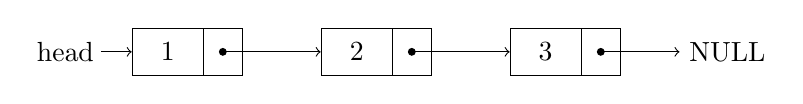
\begin{tikzpicture}[node/.style={draw,minimum width=0.9cm,minimum height=0.6cm}]
  \node at (-1.3,0) {head};
  \foreach \i/\v in {0/1,1/2,2/3} {
    \node[node] (v\i) at (\i*2.4,0) {\v};
    \node[node,minimum width=0.5cm] (n\i) at (\i*2.4+0.7,0) {};
    \fill (n\i.center) circle (0.05);
  }
  \draw[->] (-0.85,0) -- (v0.west);
  \draw[->] (n0.center) -- (v1.west);
  \draw[->] (n1.center) -- (v2.west);
  \draw[->] (n2.center) -- ++(1.0,0) node[right]{NULL};
\end{tikzpicture}
\caption{A singly linked list $1 \to 2 \to 3$.}
\end{figure}

\begin{lstlisting}[language=C]
struct Node { int val; struct Node *next; };
\end{lstlisting}

Almost every linked-list problem is solved by one of three patterns: walking with one pointer, rewiring links with a \code{prev}/\code{cur}/\code{next} trio, or running a slow and a fast pointer together.

\paragraph{Reversing a list.} Walk the list once, flipping each node's pointer to point backward.
\begin{lstlisting}[language=C]
struct Node *reverse(struct Node *head) {
    struct Node *prev = NULL, *cur = head;
    while (cur != NULL) {
        struct Node *next = cur->next;  // 1. remember the rest of the list
        cur->next = prev;               // 2. flip this node's link
        prev = cur;                     // 3. move prev forward
        cur = next;                     // 4. move cur forward
    }
    return prev;                        // prev is the new head
}
\end{lstlisting}
Trace on $1 \to 2 \to 3$: after the first pass, $1 \to$ NULL and \code{prev} $= 1$; after the second, $2 \to 1$; after the third, $3 \to 2$; \code{cur} is NULL, and the new head is 3. Time $O(n)$, extra space $O(1)$.

\paragraph{Finding the middle, and detecting a cycle.} Move \code{slow} one step and \code{fast} two steps at a time. When \code{fast} reaches the end, \code{slow} is at the middle. If the list has a cycle, \code{fast} eventually laps \code{slow} and they meet (Floyd's algorithm).
\begin{lstlisting}[language=C]
struct Node *middle(struct Node *head) {
    struct Node *slow = head, *fast = head;
    while (fast != NULL && fast->next != NULL) {
        slow = slow->next;
        fast = fast->next->next;
    }
    return slow;
}

int has_cycle(struct Node *head) {
    struct Node *slow = head, *fast = head;
    while (fast != NULL && fast->next != NULL) {
        slow = slow->next;
        fast = fast->next->next;
        if (slow == fast) return 1;
    }
    return 0;
}
\end{lstlisting}

\paragraph{Deleting nodes, with a dummy head.} Removing the first node is a special case unless you put a temporary \code{dummy} node in front of the head.
\begin{lstlisting}[language=C]
struct Node *remove_value(struct Node *head, int v) {
    struct Node dummy = { 0, head };
    struct Node *p = &dummy;
    while (p->next != NULL) {
        if (p->next->val == v) {
            struct Node *gone = p->next;
            p->next = gone->next;       // unlink it
            free(gone);
        } else {
            p = p->next;
        }
    }
    return dummy.next;
}
\end{lstlisting}

Other classic list problems use the same tools: merging two sorted lists (dummy head, pick the smaller node each step), removing the $n$th node from the end (move one pointer $n$ steps ahead, then move both), and checking whether a list is a palindrome (find the middle, reverse the second half, compare).

\section{Bit manipulation problems}

Chapter~\ref{ch:binary} explained the tricks; here they are as code.

\begin{lstlisting}[language=C]
#include <stdint.h>

// Do two 32-bit addresses fall on the same 4 KB page?
int same_page(uint32_t a, uint32_t b) {
    return (a >> 12) == (b >> 12);
}

// Mask with 1s in bits lo..hi (inclusive). Use 64-bit math so width 32 is safe.
uint32_t make_mask(int lo, int hi) {
    uint64_t width = (uint64_t)(hi - lo + 1);
    return (uint32_t)(((1ULL << width) - 1) << lo);
}

// Count the 1 bits: each step clears the lowest set bit.
int popcount(uint32_t x) {
    int count = 0;
    while (x) { x &= x - 1; count++; }
    return count;
}

// Reverse the order of the 32 bits.
uint32_t reverse_bits(uint32_t x) {
    uint32_t r = 0;
    for (int i = 0; i < 32; i++) { r = (r << 1) | (x & 1); x >>= 1; }
    return r;
}
\end{lstlisting}
To print a mask as a hex string, use \code{printf("0x\%X", m)} (or \code{sprintf} into a buffer).

\paragraph{Counting subarrays whose XOR equals $k$.} Let $P_j$ be the XOR of the first $j$ elements. The XOR of elements $i+1$ through $j$ is $P_j \oplus P_i$ (Section~\ref{sec:bitops}). It equals $k$ exactly when $P_i = P_j \oplus k$. So walk the array once, keep a hash map counting how often each prefix value has appeared, and at each step add the count of $P_j \oplus k$:
\begin{lstlisting}[language=C++]
#include <unordered_map>
#include <vector>

long long count_xor_subarrays(const std::vector<int>& a, int k) {
    std::unordered_map<int, long long> seen;
    seen[0] = 1;                   // the empty prefix
    int prefix = 0;
    long long count = 0;
    for (int x : a) {
        prefix ^= x;
        auto it = seen.find(prefix ^ k);
        if (it != seen.end()) count += it->second;
        seen[prefix]++;
    }
    return count;
}
\end{lstlisting}
This runs in $O(n)$ time instead of the $O(n^2)$ of checking every subarray. For \code{[4, 2, 2, 6, 4]} and $k = 6$ it returns 4.

\begin{onoa}
Reported Ignite coding problems include checking whether two addresses share a 4\,KB page, generating a bit mask from bit \code{lo} to bit \code{hi} as a hex string, a ``bitwise XOR subarray'' problem, a greedy problem using a heap, and, in your own assessment, a linked-list problem. Recovering an array from its prefix XORs is another reported pattern: $a_i = P_i \oplus P_{i-1}$.
\end{onoa}

\section{Complexity in one paragraph}

Big-O notation describes how running time grows with input size $n$. A rough guide to what fits in about a second: $n$ up to $10^8$ for $O(n)$; $10^5$ to $10^6$ for $O(n \log n)$ (sorting); a few thousand for $O(n^2)$. Hash maps give $O(1)$ average lookup; sorting is $O(n \log n)$; a heap (priority queue) gives $O(\log n)$ insert and remove-min, which suits greedy problems that repeatedly take the best remaining item.

\section{Hardware-flavored C}

Two features appear in firmware and drivers. \code{volatile} tells the compiler that a variable can change outside the program's control (a memory-mapped hardware register), so every read and write must actually happen. And registers are often manipulated with masks and shifts: to set a 3-bit field at bits 4--6 to value \code{v}: \code{reg = (reg \& \~{}(0x7u << 4)) | ((v \& 0x7u) << 4);}.

\section{Summary}

\begin{itemize}
  \item Know C sizes on 64-bit systems, integer division and modulo rules, and pointer arithmetic.
  \item \code{static} locals are initialized once and keep their values; macros are text substitution, so parenthesize them; post-increment uses the old value.
  \item Structs are padded for alignment: \code{\{char; void*\}} is 16 bytes on 64-bit.
  \item Linked lists: one pointer to walk, \code{prev}/\code{cur}/\code{next} to rewire, slow/fast to find the middle or a cycle, a dummy head to simplify deletions.
  \item Bit problems: shifts and masks; \code{x \& (x-1)}; prefix XOR with a hash map counts XOR subarrays in $O(n)$.
\end{itemize}

\section{Exercises}

\begin{enumerate}
  \item With \code{\#define x a+b}, \code{a = 3} and \code{b = 1}, what is \code{x*x}?
  \item A function contains \code{static int n = 0; return ++n;}. What does it return on its first four calls?
  \item On a 64-bit machine, what is \code{sizeof} of \code{struct \{ char a; double d; char b; \}}? How could you make it smaller?
  \item Write a C function that returns the number of nodes in a linked list.
  \item Trace \code{reverse} on the list $1 \to 2 \to 3 \to 4$. What does each node point to at the end?
  \item What is \code{popcount(0xF0F0)}?
  \item How many subarrays of \code{[4, 2, 2, 6, 4]} have XOR equal to 6? List them.
  \item What are \code{-7 / 2} and \code{-7 \% 2} in C?
  \item After \code{int i = 5; int j = i++ * 2;}, what are \code{i} and \code{j}?
\end{enumerate}

\subsection*{Answers}
\begin{enumerate}
  \item \code{a+b*a+b} $= 3 + 3 + 1 = 7$.
  \item 1, 2, 3, 4.
  \item \code{a} at 0, 7 bytes padding, \code{d} at 8, \code{b} at 16, 7 bytes padding: 24 bytes. Reordering as \code{\{ double d; char a; char b; \}} gives 16.
  \item One way to write it:
\begin{lstlisting}[language=C]
int length(struct Node *head) {
    int n = 0;
    for (struct Node *p = head; p != NULL; p = p->next) n++;
    return n;
}
\end{lstlisting}
  \item The result is $4 \to 3 \to 2 \to 1 \to$ NULL: node 4 is the new head and node 1 points to NULL.
  \item 8.
  \item Four: \code{[4, 2]}, \code{[4, 2, 2, 6, 4]}, \code{[2, 2, 6]}, \code{[6]}.
  \item $-3$ and $-1$.
  \item \code{i = 6}, \code{j = 10}.
\end{enumerate}
